\chapter{FUNDAMENTAÇÃO TEÓRICA}

Neste capítulo e apresentada uma revisão de assuntos relacionados na literatura, visando embasamento conceitual, para o entendimento deste trabalho.

\section{Origem dos testes na indústria}

Desde do início da indústria percebeu-se que os produtos precisam estar adequados a especificação. Produtos que são terminados com inconformidades tornam a produção mais lenta, gerando desperdícios como adaptação, retrabalho e refugo. O mesmo ocorre no processo de desenvolvimento de software, onde cada requisito deve atender as especificações solicitadas pelo cliente, caso contrário poderá ter funcionalidades inadequadas ou desnecessárias, que levam aos mesmos problemas da indústria.

A solução utilizada no secúlo XX, foi a inspeção ao final da produção. A indústria ocidental evoluiu ao fazer inspeções proativas (no estoque) e estatísticas por período de tempo. Entretanto o tempo entre a geração do erro e sua identificação diminui a capacidade de identificação da causa raíz dos problemas e de sua solução \cite{CARVALHO}.

Segundo \citeonline{HOLWEG}, em 1918 Sakichi Toyoda implantou em sua indústria de tecelagem uma máquina que verifica a linha de produção. Ao detectar anormalidades, como por exemplo a falta ou quebra da linha, a produção era parada e os operadores avisados, evitando assim a necessidade de operários para monitoramento da produção, e que o produto não atendesse a especificação. Desta maneira o tempo de identifição do problema é curto, evita vários problemas no processo de produção e aumenta as chances de análise e identificação das causas dos problemas.

Entretanto, todo o conhecimento gerado na industria oriental passou desapercebido, sem publicações científicas, até a década de 90, quando se iniciaram pesquisas a este respeito. Sendo assim, até os dias de hoje, percebe-se grandes falhas em empreendimentos nas diversas formas de indústria, inclusive na indústria de software.

\section{Prejuízos na indústria de software}

Software são desenvolvidos a mais de cinquenta anos e ainda tem grandes problemas com a qualidade e garantia de entrega. Segundo \citeonline{CHARETTE}, bilhões de dólares são gastos em projetos  que não são terminados, e 5\% a 15\% dos projetos iniciados serão abandonados antes de serem entregues ou considerados totalmente inadequados logo depois de seu término.

Desenvolver sistemas é caro, e o processo frequentemente sofre dificuldades com as metodologias adotadas, muitas delas não se adequam as atuais exigências do mercado. Por exemplo, o gerente do projeto e os desenvolvedores, devem estar sempre preparados para avaliar as demandas passadas pelos seus clientes (stakeholders) durante o processo de desenvolvimento do sistema. Na etapa de codificação, surgem constantes solicitações de modificações dos requisitos, os quais podem afetar o custo e a qualidade do software \cite{CERPA}.

O maior problema no processo de desenvolvimento é a existência de falhas no sistema, principalmente as detectáveis e previsíveis. Porém, muitas organizações ainda não consideram que a prevenção e detecção de falhas através de testes seja importante, mesmo que possam correr o risco de causar prejuízos ao cliente \cite{CHARETTE}. A tabela \ref{falhas_em_projetos} exemplifica tipos de falha em projetos de desenvolvimento de software é apresentada abaixo.

\begin{table}[ht]
	\centering
	\fontsize{8}{0}
	\caption{Percentual de projetos falhos por fator de falha \cite{CERPA}}
	\label{falhas_em_projetos}
\begin{tabular}{lccc}

\hline

\textbf{Fatores de falha em projetos de software} & \multicolumn{3}{c}{\textbf{Porcentagem de projetos (\%)}}\tabularnewline

\cline{2-4}

& \textbf{In-House} & \textbf{Outsourced} & \textbf{Geral}\tabularnewline

\hline

Data de entrega influenciou no processo & 93,9 & 90,5 & 92,9\tabularnewline

\hline

Projeto estimado por baixo & 83,7 & 76,2 & 81,4\tabularnewline

\hline

Riscos não fora reavaliados, controlados ou gerenciados & 73,4 & 80,9 & 75,7\tabularnewline

\hline

A gerência não foi recompensada por longas horas de trabalho & 81,6 & 57,1 & 74,3\tabularnewline

\hline

Tomada de decisão foi feita sem informações necessárias & 83,7 & 47,6 & 72,9\tabularnewline

\hline

A gerência teve experiência desconfortável & 83,7 & 47,6 & 72,9\tabularnewline

\hline

Clientes não envolvidos na preparação do cronograma & 69,4 & 76,2 & 71,4\tabularnewline

\hline

Risco não está incorporado no planejamento do projeto & 65,3 & 80,9 & 70,0\tabularnewline

\hline

Controle de mudanças não monitorado/negociado efetivamente & 63,3 & 85,7 & 70,0\tabularnewline

\hline

Clientes e usuários tiveram espectativas não realísticas & 69,4 & 66,7 & 68,6\tabularnewline

\hline

Processo não teve revisões ao final de cada fase & 75,5 & 47,6 & 67,1\tabularnewline

\hline

Metodologia não apropriada para o projeto & 71,4 & 52,4 & 65,7\tabularnewline

\hline

Cronograma agressivo afetou a motivação da equipe & 69,4 & 57,1 & 65,7\tabularnewline

\hline

Mudanças no escopo durante o projeto & 67,3 & 57,1 & 64,3\tabularnewline

\hline

Cronograma teve efeito negativo na vida dos elementos da equipe & 71,4 & 42,9 & 62,9\tabularnewline

\hline

Projeto com equipe inadequada para cumprir o cronograma & 63,3 & 57,1 & 61,4\tabularnewline

\hline

Equipe adicionada tardiamente para cumprir um cronograma & 61,2 & 61,9 & 61,4\tabularnewline

\hline

Clientes não dão tempo suficiente para levantar requisitos & 61,2 & 57,1 & 60,0\tabularnewline

\hline

\end{tabular}
\end{table}

\section{Filosofia de Teste de Software}

Teste de software é uma das mais importantes atividades na garantia de qualidade. Segundo \citeonline{PRESSMAN}, a atividade de teste em um projeto de software pode consumir 40\% do esforço total do mesmo e chegar a custar de três a cinco vezes mais que todas as outras etapas da engenharia de software somadas.

A definição comumente aceita da atividade de teste de software é a de que "teste de software consiste de uma série de procedimentos pré-definidos para garantir que o código faça o que ele foi projetado para fazer e não tenha nenhum comportamento não desejado". Porém, \citeonline{MYERS}, aponta para o fato de que o objetivo primário de um teste de software é encontrar erros no código e não provar que o programa atinge aos objetivos: "Teste de software é o processo de se executar um programa com o propósito de descobrir erros". 

Muitos programadores assumem uma definição menos eficiente sobre a atividade de teste:

\begin{itemize}
\item A atividade de teste é o processo de demonstrar a inexistência de erros no software
\end{itemize}

Esse pensamento comum é inapropriado pois apesar da atividade de teste poder descobrir defeitos no software, ela é incapaz de mostrar a inexistência destes. No mundo real, é impraticável criar casos de teste para todas as combinações e cenários possíveis para aplicações mais complexas.

\begin{itemize}
\item O propósito da atividade de teste é mostrar que um programa executa suas funções corretamente.
\end{itemize}

Esta definição pode ser considerada incompleta pois mesmo que um programa atinja os objetivos para o qual foi projetado, ainda pode conter erros caso apresente funcionalidades adicionais.

\begin{itemize}
\item Teste de software é o processo de garantir que um programa faz o que foi projetado para fazer.
\end{itemize}

Apesar de uma atividade de teste bem executada poder demonstrar a conformidade entre os requisitos do cliente e as funcionalidades implementadas no software, este é um benefício secundário. Como qualquer outra atividade no processo de desenvolvimento, testes também devem agregar valor ao software, e portanto é importante encontrar defeitos. Neste sentido, a qualidade da atividade de teste será diretamente proporcial ao esforço em encontrar defeitos.

Por tudo isso, percebe-se que os testes de software cumprem uma função ética no processo de desenvolvimento, evitando prejuízos para as organizações ou pessoas. Um exemplo claro disso, é a responsabilidade atribuída ao desenvolvedor do algoritmo presente em um marca-passo, onde qualquer falha pode causar graves prejuízos ao usuário.

Portanto, para conduzir os testes efetivamente, existe toda uma complexidade advinda da variedade de algorítmos que precisarão ser testados. Várias técnicas propostas para endereçar os testes de algorítmos são apresentadas nos tópico a seguir.

\section{Tipos de testes de software}

...

\section{Formato \textit{YAML}}
\label{sec:yaml}

O \textit{YAML} é um formato de serialização de dados que pode ser facilmente entendível por humanos e ao mesmo tempo é flexível e facilmente manipulável. Ele aceita representação para as estruturas de listas, dicionários e valores simples, como texto e inteiros \cite{YAML}.

Além disso, este formato utiliza uma notação baseada em indentação e um conjunto de caracteres para demarcar sua estrutura. Abaixo serão listadas algumas outras características deste formato.

\begin{itemize}
\item A estrutura do documento é composto por indentação com espaços em branco e não é permitido o uso de caracteres de tabulação para a indentação.

\item Os valores simples não levam as aspas, mas podem ser incluídas as aspas duplas ou aspas simples.

\item Os membros das listas são encabeçados por um traço nos títulos e com um membro em cada linha, ou entre colchetes e separados por uma vírgula e espaço.
\end{itemize}

O Código \ref{lst:codigo21} exemplifica as caracteristicas descritas anteriormente.

{\singlespace
\begin{lstlisting}[caption=Estrutura do código \textit{YAML},language=bash,label={lst:codigo21}]
titulo: "Exemplo de listas"
data: Julho de 2012

listagem_1: [Tiago, Natanael]

listagem_2:
  - Tiago
  - Natanael
\end{lstlisting}
}


\section{JavaScript}

JavaScript (JS) surgiu em 1995, com o objetivo de validar a entrada de dados em páginas web, pois neste período nem todos os dados eram tratados pelo servidor. A capacidade de lidar com algumas validações básicas no cliente, era uma característica nova e excitante, num momento em que o uso de modems de telefone estava crescendo, e a lenta velocidade das conexões tornavam o acesso a web um exercício de paciência \cite{ZAKAS}.

Segundo \citeonline{PIRES}, JS é uma linguagem de programação, pequena, leve, orientada a objetos e multi-plataforma (Código \ref{lst:codigo22}). Mais conhecida como uma linguagem de script para páginas web, mas também muito bem utilizada em dispositivos móveis modernos, como celulares e tablets. Hoje em dia, JS é uma linguagem que pode ser utilizada em qualquer aspecto, desde aplicações no lado cliente (aplicações de front-end), como do lado servidor (aplicações server-side).

{\singlespace
\begin{lstlisting}[caption=Classe Pessoa em \textit{JavaScript},language=Java,label={lst:codigo22}]
<script language="javascript">
function Pessoa () {
    var nome;
    var sobrenome;
    
    this.getNome = getNome;
    this.getSobrenome = getSobrenome;
    this.setNome = setNome;
    this.setSobrenome = setSobrenome;
    this.nomeCompleto = nomeCompleto;
    
    function getNome () {
        return nome;
    }
    
    function getSobrenome () {
        return sobrenome;
    }
    
    function setNome (_nome) {
        nome = _nome;
    }
    
    function setSobrenome (_sobrenome) {
        sobrenome = _sobrenome;
    }
    
    function nomeCompleto () {
        return getNome() + " " + getSobrenome();
    }
}
</script>
\end{lstlisting}
}

Portanto, esta linguagem pode interagir com todo conteúdo da página e a janela do navegador, sem realizar requisições ao servidor da aplicação, desta forma oferece uma dinâmica maior às páginas, maior velocidade ao usuário e maior flexibilidade ao programador.

\section{\textit{jQuery}}
\label{sec:jquery}

Nos dias de hoje a \textit{internet} é um ambiente dinâmico, e os seus usuários exigem cada vez mais interatividade e estilo. Para construir interessantes sites interativos, os desenvolvedores voltam-se para o uso bibliotecas \textit{JavaScript} como \textit{jQuery}. Esta biblioteca permite automatizar tarefas comuns e simplificar as complicadas. Uma das razões para a popularidade do \textit{jQuery} é sua capacidade de ajudar em uma ampla gama de tarefas.

Segundo \citeonline{CHAFFER} muitos dos conceitos da biblioteca são baseados na estrutura do código \textit{HTML} e \textit{Cascading Style Sheets} (CSS). Suas principais características podem nos ajudar a realizar as seguintes tarefas:

\begin{itemize}
\item Acessar os elementos da página: Sem utilizar uma biblioteca \textit{JavaScript} que facilite a seleção de elementos da página, desenvolvedores precisam escrever complexos scripts utilizando a estrutura do \textit{Document Object Model} (DOM). Através desta biblioteca, é possível utilizar um eficiente mecanismo de seleção dos elementos.

\begin{center}
\textit{\$('div.content').find('p');}
\end{center}

\item Alterar a aparência da página: CSS oferece uma poderosa maneira de alterar a aparência de páginas web. Com \textit{jQuery} os desenvolvedores podem alterar dinamicamente as propriedades do CSS da página, mesmo que ela já tenha sido carregada.

\begin{center}
\textit{\$('ul > li:first').addClass('active');}
\end{center}

\item Manipular o conteúdo da página: \textit{jQuery} pode modificar o conteúdo da página sem maiores problemas. É possível alterar textos, adicionar ou trocar imagens, re-ordenar listas e até adicionar novos elementos na página, tudo isso com uma \textit{Application Programming Interface} (API) fácil de usar \cite{JQUERY-API}.

\begin{center}
\textit{\$('\#container').append('<pre>News</pre>');}
\end{center}

\item Responder a interação do usuário: A biblioteca oferece uma maneira simples de interceptar a vasta gama de eventos que o usuário pode disparar, como por exemplo, o evento de clicar em um \textit{link}.

\begin{center}
\textit{\$('button.show-details').click(function() \{ \$('div.details').show(); \});}
\end{center}

\item Executar requisições assíncronas: Esta técnica é chamada de AJAX, o que significa \textit{Asynchronous JavaScript and XML}, a qual possibilita a comunicação cliente-servidor. Desta maneira o desenvolvedor pode executar chamadas ao servidor sem recarregar a página.

\begin{center}
\textit{\$('div.details').load('more.html \#content');}
\end{center}

\item Solucionar incompatibilidades de navegadores: Esta biblioteca é \textit{cross-browser}, o que significa a total compatibilidade de sua API com os atuais navegadores.
\end{itemize}

Portanto, a utilização desta biblioteca facilita o desenvolvimento de aplicações web e diminui a probabilidade de erros, causados pela divergência de padrões existentes entre os navegadores.

\section{\textit{Amberjack}}
\label{sec:amberjack}

\textit{Amberjack} (AJ) é uma biblioteca de código aberto que você pode usar para criar \textit{tours} - tutoriais guiados - que orientam os visitantes do seu site. A idéia básica é explicar as páginas existentes do seu site através de um texto (como este). O texto explicativo é exibido em uma caixa de diálogo uma camada acima da sua página \textit{web} (Figura \ref{figura_22}). AJ foi criado com ênfase na flexibilidade e na facilidade de customização.

\begin{figure}[ht]
    \centering
    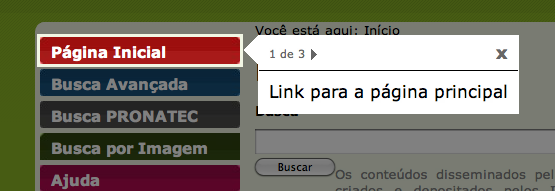
\includegraphics[width=0.9 \textwidth]{figuras/figura_33}
    \caption{\textit{Tour} gerado pela biblioteca \textit{Amberjack}}
    \label{figura_22}
\end{figure}

Para utilizar esta biblioteca não é necessário amplo conhecimento de \textit{JavaScript}, você só precisa adicionar um código \textit{HTML} a sua página web. Este código descreve cada passo que será realizado na página. O código é organizado por um estrutura de "div" aninhados e atributos que descrevem propriedades do cenário (Código \ref{lst:codigo22}).

{\singlespace
\begin{lstlisting}[caption=Estrutura do código \textit{HTML} do \textit{Amberjack},language=HTML,label={lst:codigo23}]
<div class="ajTourDef" id="MeuExemplo" style="display:none" title="http://feedback.exemplo.com/">
  <div title="http://exemplo.com/">
    <div title="id:'elemento1',padding:0,trbl:'ltb'">
      <strong>Primeiro passo</strong>
      <br />Primeiro passo na página inicial
    </div>
    <div title="id:'elemento2',padding:0,trbl:'ltb'">
      Segundo passo
      <br />Próximo passo será em outra página.
    </div>    
  </div>
  <div title="http://exemplo.com/noticias">
    <div title="id:'markerColor',padding:0,trbl:'ltb'">
      <strong>Fim do exemplo</strong>
      <br />Página de notícias.
    </div>
  </div>
</div>
\end{lstlisting}
}

A primeira linha define uma ``div'' responsável pelo tutorial. Nesta ``div'' são definidos dois importantes atributos, id e title. O id é o identificador do tutorial, o qual deve ser utilizado para iniciá-lo, já o title define a url que o usuário será redirecionado ao terminar o tutorial.

Nas linhas 2 e 12, são criadas as ``div'' que definem o contexto no qual os passos serão realizados. O atributo title define a url na qual os passos serão executados.

Dentro de cada uma destas ``div'' que estabelecem o contexto de execução, são criadas as estruturas finais. Cada ``div'' que encontra-se dentro de um contexto, tem dois importantes atributos, id e trbl. Eles são reponsáveis por definir qual elemento da página será destacado e qual será a posição da caixa de diálogo \cite{AJ}. O conteúdo de cada uma delas será o texto exibido no \textit{tour}.

Por fim, após definir todos os cenários que deseja inserir um \textit{tour}, o mesmo pode ser iniciado a partir da passagem de um parâmetro na url:

\begin{center}
\textit{http://meuexemplo.com/?tourId=MeuExemplo\&skinId=Safari}
\end{center}